\newpage
\phantomsection
{\bfseries IRSTI 20.53.01}
\hfill {\bfseries \href{https://doi.org/10.58805/kazutb.v.2.23-404}{https://doi.org/10.58805/kazutb.v.2.23-404}}

\sectionwithauthors{D. Kair}{COMPARISON AND ANALYSIS OF DIFFERENT MACHINE LEARNING METHODS ON
WEATHER TEMPERATURE PREDICTIONS BASED ON THE OPEN DATA}

\begin{center}
{\bfseries D. Kair}

Kazakh-British Technical University, Almaty, Kazakhstan,

e-mail: danikkair@gmail.com
\end{center}

The database obtained from the rp5 data archive is provided by the LLC
"Weather Schedule" and represents the collected information about
weather conditions in all parts of the world, describing temperature,
clouds, and precipitation, and is available for analysis to everyone.
Data is collected every 3 hours, which provides valuable data from day
to day. Many of these features are optional and dependent on time, like
maximum temperature during night time, also vision range during night
always equals zero, etc. The purpose of this study is to create a
solution, that can deal with missing data, and to find an important
machine-learning combination for weather prediction. It needs to be
mentioned that a study should be done on open data since it doesn't have
any presumptions inside. With work on raw and open data, we can try to
establish new rules in weather prediction modeling and find meaningful
solutions for Kazakhstani society. For this research, algorithms for
implementing prediction models were used from the scikitlearn Python
library. It contains Gradient Boosting Regressor, XGBoost, CatBoost,
Linear Regression, Bayesian Ridge, etc. Applied machine learning
algorithms were evaluated based on different approaches: from various
data preprocessing ideas to selecting best best-performing model with
better results and optimizing it to achieve the possible maximum in
predictions. The key course of this study is to help find a way to the
optimal approach to weather prediction problems and analysis by the way,
which current tendencies can look at it.

{\bfseries Keywords}: machine learning, weather, prediction model,
CatBoost, Linear Regression, ElasticNet, LightGBM, forecasting.

\begin{center}
{\large\bfseries АШЫҚ МӘЛІМЕТТЕР НЕГІЗІНДЕ АУА-АУРА ТЕМПЕРАТУРАСЫН БОЛЖАУ ҮШІН
ТҮРЛІ МАШИНАЛЫҚ ОҚУ ӘДІСТЕРІН САЛЫСТЫРУ ЖӘНЕ ТАЛДАУ}

{\bfseries Д. Каир}

Қазақстан-Британ техникалық университеті, Алматы, Қазақстан,

e-mail: danikkair@gmail.com
\end{center}

Rp5 деректер мұрағатынан алынған мәліметтер базасы «Ауа-Райы кестесі»
ЖШС-мен қамтамасыз етілген және температураны, бұлттылықты және
жауын-шашынды сипаттайтын әлемнің барлық бөліктеріндегі ауа-райы туралы
жиналған ақпарат болып табылады және барлығына талдау үшін қол жетімді.
Деректер әр 3 сағат сайын жиналады, бұл күн сайын құнды мәліметтер алуға
мүмкіндік береді. Бұл мүмкіндіктердің көпшілігі міндетті емес және
уақытқа байланысты, мысалы, түнгі максималды температура, түнде көру
диапазоны әрқашан нөлге тең және т.б. Бұл зерттеудің мақсаты -
жетіспейтін деректермен жұмыс істей алатын шешім жасау және ауа-райын
болжау үшін машиналық оқытудың маңызды комбинациясын табу. Айта кету
керек, зерттеу ашық деректерде жүргізілуі керек, өйткені оларда ешқандай
алғышарттар жоқ. Шикі және ашық деректермен жұмыс жасай отырып, біз ауа
райы болжамын модельдеуде жаңа ережелерді белгілеуге және қазақстандық
қоғам үшін маңызды шешімдерді табуға тырыса аламыз. Бұл зерттеу үшін
scikitlearn Python кітапханасынан болжау модельдерін енгізу алгоритмдері
қолданылды. Онда Gradient Boosting Regressor, XGBoost, CatBoost, Linear
Regression, Bayesian Ridge және т.б. регрессорлар бар. Қолданылатын
Машиналық оқыту алгоритмдері әртүрлі тәсілдер негізінде бағаланды:
деректерді алдын ала өңдеудің әртүрлі идеяларынан бастап ең жақсы
нәтижелерге қол жеткізетін ең жақсы модельді таңдауға және болжамдарда
мүмкін максимумға жету үшін оны оңтайландыруға дейін. Бұл зерттеудің
негізгі бағыты - ауа-райын болжау мәселелерін шешудің оңтайлы тәсілін
табуға көмектесу және қазіргі тенденциялар бұған қалай қарайтынын
талдау.

{\bfseries Түйін сөздер:} машиналық оқыту, ауа-райы, болжау моделі,
CatBoost, Linear Regression, ElasticNet, LightGBM, болжау.

\begin{center}
{\large\bfseries СРАВНЕНИЕ И АНАЛИЗ РАЗНЫХ МЕТОДОВ МАШИННОГО ОБУЧЕНИЯ ДЛЯ ПРОГНОЗИРОВАНИЯ ТЕМПЕРАТУРЫ ПОГОДЫ НА ОСНОВЕ ОТКРЫТЫХ ДАННЫХ}

{\bfseries Д. Каир}

Казахстанско-Британский Технический Университет, Алматы, Казахстан,

e-mail: danikkair@gmail.com
\end{center}

База данных, полученная из архива данных rp5, предоставлена ООО
"Расписание погоды" и представляет собой собранную информацию о погодных
условиях во всех частях света, описывающую температуру, облачность и
осадки, и доступна для анализа всем желающим. Данные собираются каждые 3
часа, что позволяет получать ценные сведения изо дня в день. Многие из
этих функций являются необязательными и зависят от времени, например,
максимальная температура в ночное время, дальность видимости ночью
всегда равна нулю и т. д. Цель данного исследования - создать решение,
которое сможет справиться с отсутствующими данными, и найти важную
комбинацию машинного обучения для предсказания погоды. Следует отметить,
что исследование должно проводиться на открытых данных, поскольку они не
содержат никаких предпосылок. Работая с сырыми и открытыми данными, мы
можем попытаться установить новые правила в моделировании прогноза
погоды и найти значимые решения для казахстанского общества. Для данного
исследования были использованы алгоритмы реализации моделей
прогнозирования из библиотеки scikitlearn Python. Она содержит
регрессоры Gradient Boosting Regressor, XGBoost, CatBoost, Linear
Regression, Bayesian Ridge и другие. Применяемые алгоритмы машинного
обучения оценивались на основе различных подходов: от различных идей
предварительной обработки данных до выбора лучшей модели с лучшими
результатами и ее оптимизации для достижения возможного максимума в
прогнозах. Ключевым направлением данного исследования является помощь в
поиске оптимального подхода к решению задач прогнозирования погоды и
анализ того, как на это могут смотреть современные тенденции.

{\bfseries Ключевые слова:} машинное обучение, погода, модель
прогнозирования, CatBoost, Linear Regression, ElasticNet, LightGBM,
прогнозирование.

\begin{multicols}{2}
{\bfseries Introduction}. Weather forecasting is an essential aspect of our
daily lives, as it helps us prepare for and manage the impact of weather
conditions. While weather forecasting has improved in recent years,
there are still challenges in creating accurate and timely forecasts.
One of the key challenges is the collection and analysis of data from
different weather stations to generate numerical forecasts. The current
approaches for collecting and analyzing data are often limited and may
not be optimized for weather forecasting tasks. {[}1{]} As such, there
is a need for a numerical forecast generating system that uses open data
from weather stations, collects and analyzes different data, creates
logical connections between events, and generates numerical data that
can be used in future weather forecasting. Previous studies have shown
the potential {[}2{]} of using open data from weather stations and
machine learning algorithms in weather forecasting. {[}3{]} However,
there are still gaps in these approaches, including optimization for
weather forecasting tasks and flexibility to turn into a near-real-time
system. To address these gaps, the proposed system will collect and
analyze different data, create logical connections between events, and
generate numerical data that can be used in future weather forecasting.
The current approach for weather forecasting in Almaty faces several
significant problems that limit its effectiveness in accurately
predicting weather patterns and thunderstorm activity. These problems
include:

1. \emph{Insufficient Spatial Resolution:} The existing meteorological
models used for forecasting in Almaty often have a coarse spatial
resolution. This limitation hampers their ability to capture local
variations in topography and atmospheric conditions accurately. As a
result, important microscale features that significantly influence
weather patterns and thunderstorm development, such as mountainous
terrain and localized wind patterns, are not adequately represented in
the overall forecasts {[}4{]}.

2. \emph{Inadequate Data Assimilation:} Accurate weather forecasting
relies heavily on assimilating various types of observational data,
such as satellite images, radar data, and ground-based measurements.
However, the current approach in Almaty struggles with effectively
incorporating these diverse data sources into the forecasting models.
This limitation leads to biases and errors in the initial conditions
of the models, which subsequently propagate and amplify throughout the
forecast period {[}5{]}.

3. \emph{Limited Representation of Atmospheric Processes:} Traditional
meteorological models used in Almaty often simplify or neglect certain
atmospheric processes that are crucial for accurate weather
prediction. For instance, convective processes that drive thunderstorm
activity are challenging to simulate accurately due to their highly
nonlinear nature. The current approach may not adequately capture the
complex interactions between moisture, temperature, and wind fields,
leading to inaccurate forecasts of thunderstorm occurrence, intensity,
and duration {[}6{]}.

4. \emph{Lack of Consideration for Local Effects:}
Almaty\textquotesingle s weather patterns are influenced by local
factors such as the city\textquotesingle s urban heat island effect,
lake-breeze circulation, and the proximity to mountain ranges.
However, the current approach may not adequately account for these
local effects, leading to biases in the forecasts. For example, the
urban heat island effect can significantly impact temperature
gradients, wind patterns, and the initiation and intensity of
thunderstorms, but it may be inadequately represented in the current
forecasting models {[}7{]}.

Our research is based on the database of weather measurements from rp5
presented by the LLC "Weather Schedule". It contains worldwide data for
open usage and is updated every 3 hours. Here, historical data for
Almaty City was obtained to train our model. Some data is missed due to
logical reasons, like night maximum temperature (it is obtained in
intervals) and some data is logically unnecessary, like type of clouds.
In our research, we will try to deal with different types of data,
implement it, and analyze it. The following table contains data
explanation.
\end{multicols}

\begin{table}[H]
\caption*{Table 1 -- The embeddings for each column}
\centering
\begin{tabular}{|l|p{0.8\textwidth}|}
\hline
name & description                                                                                                                                                                    \\ \hline
T    & Air Temperature (degrees Celsius) at a height of 2 meters above the ground                                                                                                     \\ \hline
Po   & Atmospheric pressure at the station level (millimeters of mercury)                                                                                                             \\ \hline
P    & Atmospheric pressure reduced to mean sea level (millimeters of mercury)                                                                                                        \\ \hline
Pa   & Baric trend: change in atmospheric pressure over the last three hours (millimeters of mercury)                                                                                 \\ \hline
U    & Relative humidity (\%) at a height of 2 meters above the ground                                                                                                                \\ \hline
DD   & Wind direction (points) at an altitude of 10-12 meters above the Earth's surface, averaged over the 10-minute period immediately preceding the observation period              \\ \hline
Ff   & Wind speed at an altitude of 10-12 meters above the Earth's surface, averaged over the 10- minute period immediately preceding the observation period (meters per second)      \\ \hline
ff10 & The maximum value of the wind gust at altitude 10-12 meters above the Earth's surface in the 10-minute period immediately preceding the observation period (meters per second) \\ \hline
ff3  & The maximum value of the wind gust at altitude 10-12 meters above the earth's surface in the period between deadlines (meters per second)                                      \\ \hline
WW   & Current weather reported from the weather station                                                                                                                              \\ \hline
Tn   & Minimum air temperature (degrees Celsius) for the past period (no more than 12 hours)                                                                                          \\ \hline
Tx   & Maximum air temperature (degrees Celsius) for the past period (no more than 12 hours)                                                                                          \\ \hline
VV   & Horizontal visibility range (km)                                                                                                                                               \\ \hline
Td   & Dew point temperature at a height of 2 meters above the earth's surface (degrees Celsius)                                                                                      \\ \hline
\end{tabular}
\end{table}

\begin{multicols}{2}
{\bfseries Literature review.} Addressing these problems and improving the
accuracy of weather and thunderstorm forecasts in Almaty requires the
development of an advanced numerical forecasting model that incorporates
higher spatial resolution, improved data assimilation techniques, and
better representation of atmospheric processes. By overcoming these
limitations, the forecasting system can provide more precise and
reliable information, enabling stakeholders and decision-makers in
Almaty to effectively prepare for and mitigate the impacts of severe
weather events.

Previous research has shown that open data from weather stations can be
used to improve weather forecasting accuracy. For instance, in a study
by {[}8{]}, open data from weather stations were used to improve
forecasting accuracy in urban areas. The researchers found that
incorporating open data from weather stations led to a more accurate
forecast of temperature, humidity, and wind speed. Similarly, a study by
{[}9{]} found that autoregression combined with machine learning
algorithms enables compelling multi-step predictions of these NWP wind
velocity residuals. Linear autoregression is proven to achieve fast and
competitive forecasts with rigorous statistical approaches. The
superiority of the statistical method for machine learning is further
demonstrated by the fact that the residual series are considerably
stochastic and sophisticated algorithms resulting in overfitting.

Machine learning algorithms have also been explored in weather
forecasting research. {[}10{]} used machine learning algorithms to
improve short-term wind speed forecasting. The study found that machine
learning algorithms could be used to generate more accurate wind speed
forecasts. In another study, {[}11{]} compared the performance of
different machine learning algorithms in thunderstorm frequency
prediction. The researchers found that different hybrid machine learning
algorithms could generate accurate thunderstorm frequency forecasts.
Also, in {[}12{]} researchers found that data collected from
multi-observation meteorological and data collected from GNSS lead to
different results in terms of the NWP (Numerical Weather Prediction)
model. Some studies also included a mathematical basis for themselves,
meaning that weather forecast needs a combination of numeric and
probabilistic models {[}13{]}. Atmospheric weather prediction was
achieved by using a wide variety of weather figure methods {[}14{]}.
Here {[}15{]}, researchers decided to use the idea of mathematical and
statistical decision tree and conditions vide confusion matrix for more
appropriate and accurate forecasting using Big Data. Even hybrid
approach already exists {[}16{]}: researchers decided to create a hybrid
Global Climate Model, where Hybrid model gave almost the same results as
the normal one, but optimization in their research helped to achieve
huge results in model speed, what opens a new room for model
improvements.

It is also clearly seen that weather prediction can be achieved in real
time by using Internet of Things and Machine Learning in combination
{[}17{]}. There, light intensity sensors, humidity sensors and different
modules have been used. As for Machine Learning, authors decided to use
a logistic regression model to set up an environment.

Researchers from China decided to explore DLWP (Deep Learning based
Weather Prediction) in compare with Numerical Weather Prediction, in
which we are interested. During their survey, they focused not only
Neural Networks architectures for various types of data, but also made a
comparative analysis from different perspectives of spatio-temporal
scales, datasets and benchmarks. They have found out that Deep Learning
also can be considered suitable and reasonable tool for analyzing the
characteristics of time series connected with weather {[}18{]}.

We also want to mention local characteristics of area as an important
feature. For example, short term weather prediction has been done in Sri
Lanka, where as a result local tropic climate has affect onto weather
prediction patterns. For them, it was tremendously challenging due to
high temperature and sudden atmospheric circulations. It was important
to understand how to deal with local features on this example, since
Almaty also has exclusive features, like unique earth relief and is
surrounded by mountains.

Despite the potential o f using open data from weather stations and
machine learning algorithms in weather forecasting, there are still some
gaps in these approaches. Some of these approaches may not be optimized
for weather forecasting tasks, which can lead to inaccurate forecasts.
Additionally, some approaches may not be flexible enough to be turned
into a near-real-time system, which can hinder their usefulness in
providing timely forecasts. As such, there is a need for a system that
can optimize these approaches for weather forecasting.

Data

The dataset contains 29 columns of different data. In a Table 1 we
mentioned only used ones, since many columns consists of unnecessary in
prediction data. Some data became unnecessary due to overly biased
results, some due to unimportance (type of clouds), some due to lots of
missed values.
\end{multicols}

\begin{figure}[H]
	\centering
	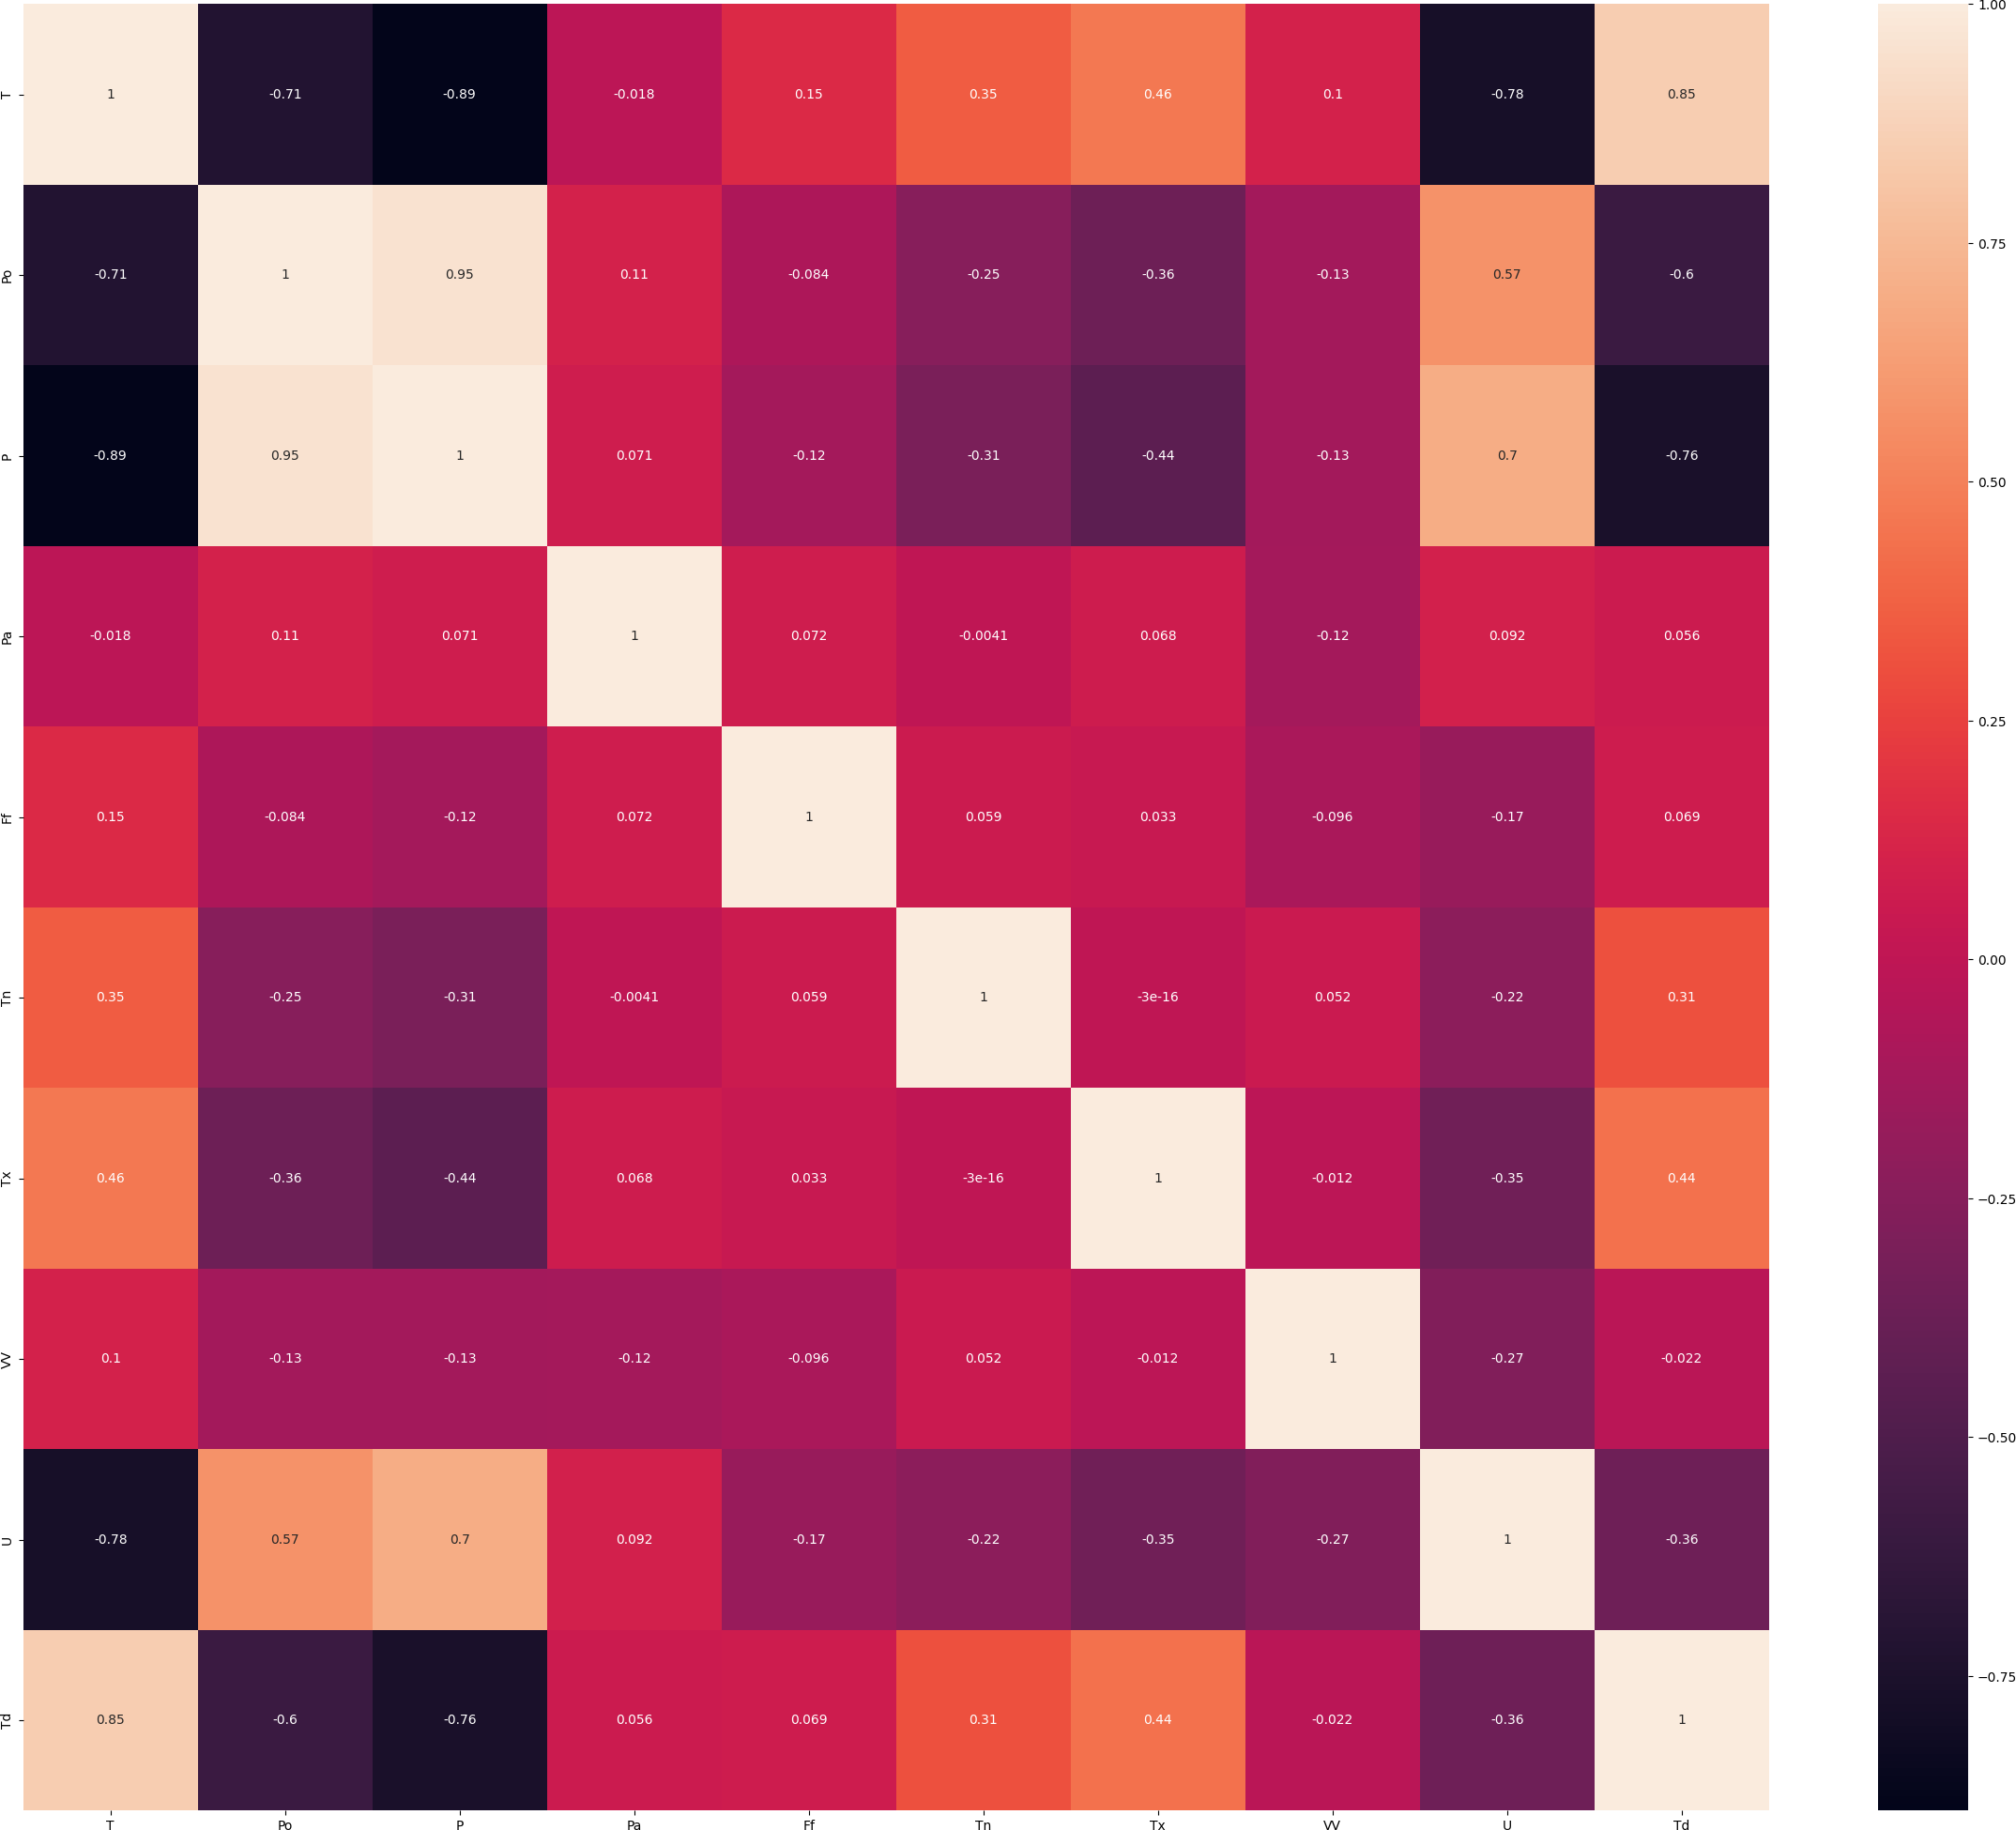
\includegraphics[width=0.8\textwidth]{assets/36}
	\caption*{Figure 1 -- Correlation heatmap for all numerical and categorical features}
\end{figure}

\begin{multicols}{2}
After logical analysis, we began analyzing attributes by plotting the
correlation heatmap for all remaining features in order to obtain the
significant ones to the task of weather prediction (see Figure 1). To
plot correlation heatmap we used seaborn Python library and Pandas
built-in .corr method, which can use Spearman rank correlation,
Pearson(standard) correlation coefficient, and Kendall Tau correlation
coefficient. According to this data it was decided to left only
following columns: \textquotesingle T\textquotesingle,
\textquotesingle Po\textquotesingle, \textquotesingle P\textquotesingle,
\textquotesingle Pa\textquotesingle,
\textquotesingle Ff\textquotesingle,
\textquotesingle Tn\textquotesingle,
\textquotesingle Tx\textquotesingle,
\textquotesingle VV\textquotesingle, \textquotesingle U\textquotesingle,
\textquotesingle Td\textquotesingle. Since their pairwise correlation is
between -0.1 and 0.1, and some of them considered to be used due to
better overall model performance with them.
\end{multicols}

\begin{table}[H]
\caption*{Table 2 - Number of rows with missing values for given attributes}
\centering
\begin{tabular}{|l|l|}
\hline
Column & Rows 				with NaN value \\ \hline
T      & 0                       \\ \hline
Po     & 1                       \\ \hline
P      & 1                       \\ \hline
Pa     & 4                       \\ \hline
Ff     & 0                       \\ \hline
Tn     & 2568                    \\ \hline
Tx     & 2205                    \\ \hline
VV     & 1331                    \\ \hline
U      & 7                       \\ \hline
Td     & 7                       \\ \hline
\end{tabular}
\end{table}

\begin{multicols}{2}
For left columns, we decided to approach to another method of data
preprocessing -- by clearing missing values. As shown in Table 2 -- only
2 of left columns are full, while others need to handle missing data.
For numerical columns using mean value gave us the best performance, but
for rows with words, we considered to transfer them into related values.
For example, when speed of wind wasn't a number, dataset contained
`calm' instead of number, as a part of data preprocessing, we changed by
ourselves it into zeros, result became better than by deleting rows with
them.

In a result, we split data into two sets: train and test. Train dataset
contained data from 1\textsuperscript{st} of April 2022 to
31\textsuperscript{st} of March 2023. Test dataset was from
1\textsuperscript{st} of April 2023 to 31\textsuperscript{st} of March
2024. Such decision was chosen due to similarity of time intervals,
containing similar days of year.


Methods and materials. First step was to scale our data for better model
performance. We decided to use MinMaxScaler from SkLearn python library.
MinMaxScaler scales all the data features in the range {[}0, 1{]} or
else in the range {[}-1, 1{]} if there are negative values in the
dataset. In conclusion, model with scaled values performed much better
than unscaled one, what can be seen in a final result.


Second step was to choose best-performing general model, which will be
used in a future. So, during the training and prediction phases of
study, we were able to inspect performance of several popular machine
learning techniques, connected with regression: Gradient Boosting
Regressor, Random Forest, Linear Regression, ElasticNet, SGD Regressor,
Bayesian Ridge, Support Vector Regressor, CatBoost, Kernel Ridge,
XGBoost and LightGBM. Here is a brief explanation of each model:

\emph{{\bfseries Gradient Boosting Regressor:}} Gradient Boosting is an
ensemble learning method that builds a strong predictive model by
combining multiple weak models, usually decision trees. It works by
iteratively adding new models that focus on the residuals of the
previous models, gradually improving the overall predictions.

\emph{{\bfseries Random Forest:}} Random Forest is another ensemble
learning method that constructs multiple decision trees and combines
their predictions. Each decision tree is trained on a random subset of
the data and features. The final prediction is obtained by averaging the
predictions of all the individual trees.

\emph{{\bfseries Linear Regression:}} Linear Regression is a simple and
widely-used linear modeling technique. It assumes a linear relationship
between the input features and the target variable. The model fits a
line to the data that minimizes the sum of squared differences between
the observed and predicted values.

\emph{{\bfseries ElasticNet:}} ElasticNet is a linear regression model that
combines both L1 (Lasso) and L2 (Ridge) regularization penalties. It is
useful when dealing with high-dimensional datasets and aims to find a
balance between feature selection (L1 regularization) and handling
multicollinearity (L2 regularization).

\emph{{\bfseries SGD Regressor:}} Stochastic Gradient Descent (SGD) is an
iterative optimization algorithm used for linear regression. It updates
the model\textquotesingle s parameters based on a randomly selected
subset of the training data at each iteration, making it suitable for
large-scale datasets.

\emph{{\bfseries Bayesian Ridge:}} Bayesian Ridge regression is a Bayesian
statistical model that combines a prior distribution with the likelihood
function to estimate the model parameters. It provides a probabilistic
framework for linear regression and automatically determines the
regularization strength.

\emph{{\bfseries Support Vector Regressor:}} Support Vector Regression
(SVR) is a variant of Support Vector Machines adapted for regression
problems. It finds a hyperplane that best fits the data while
considering a margin that controls the trade-off between fitting the
data and allowing some deviations.

\emph{{\bfseries CatBoost:}} CatBoost is a gradient boosting algorithm that
is known for its ability to handle categorical variables efficiently. It
incorporates a range of advanced techniques, such as ordered boosting
and categorical feature embeddings, to improve predictive performance.

\emph{{\bfseries Kernel Ridge:}} Kernel Ridge regression combines ridge
regression with the kernel trick to perform non-linear regression. It
uses a kernel function to map the input features into a
higher-dimensional space, where linear regression is applied. It is
effective for capturing complex patterns in the data.

\emph{{\bfseries XGBoost:}} XGBoost is an optimized gradient boosting
algorithm that is highly efficient and scalable. It uses a combination
of tree-based models and gradient boosting techniques to achieve
accurate predictions. XGBoost is known for its speed and performance on
structured data.

\emph{{\bfseries LightGBM:}} LightGBM is another gradient boosting
framework that is designed to be fast and memory-efficient. It uses a
special type of decision tree called the "leaf-wise" tree, which can
lead to better accuracy with less memory consumption compared to
traditional gradient boosting methods.

\begin{table}[H]
\caption*{Table 3 -- Model performance results after test training}
\centering
\begin{tabular}{|l|l|}
\hline
Model name & Mean Squared Error \\ \hline
GB Regressor & 0.740616 \\ \hline
RF Regressor & 0.602757 \\ \hline
Linear Regression & 3.430981 \\ \hline
ElasticNet & 107.581766 \\ \hline
SGD Regressor & 2.586797 \\ \hline
Bayesian Ridge & 3.427670 \\ \hline
SVR & 2.530081 \\ \hline
CatBoost & 0.240654 \\ \hline
Kernel Ridge & 2.453900 \\ \hline
XGBoost & 0.678889 \\ \hline
LightGBM & 0.637373 \\ \hline
\end{tabular}
\end{table}

CatBoost model performed better than any other one with a mean squared
error result of 0.240654. In our research we decided to further maintain
CatBoost as main model.

Also, we tried to optimize it with Grid Search Cross-Validation. It was
applied to CatBoostRegressor to find the best hyperparameters for our
final model. It seems that the parameter tuning yielded worse results as
compared to the default setting. Therefore, default model will be used
without any hyperparameter tuning.

Results and Discussion. In result, we can see that XGBoost with LightGBM
showed a bit worse performance. This means that for our data this
gradient boosting algorithms suits best. But in a result, we needed only
one, without any hybrid models. The next step was to tune model
parameters to achieve better performance, but after tests, it has been
found that the parameter tuning yielded worse results as compared to the
default setting. Therefore, default model used without any
hyperparameter tuning. After that, we trained and tested our final
model. When we applied the needed settings and solutions, we found out
R2 score of 0.97237. In this study, the authors use the R2 score as a
main indicator of accuracy. While R2 score of 1 means ideal prediction,
\textasciitilde0.97 means that our prediction model gave us strong
results. Authors can observe the difference between forecasting results
of data before and after outlier removal with \emph{different}
attributes in Table 2. Also, it is clearly seen that CatBoost performs
much better without any model optimization and better suits to weather
prediction task.


To conduct results, authors decided to test out Feature and SHAP
importances. We made several tests and applied different weights to our
model features. In a result, authors got a necessary for further
research information, which contained that Td, U, P, Po are important
attributes for our model due to results of Feature importance test. SHAP
results were a bit different, they contained Tx and Tn features in
addition to previous ones. So, it can be seen that temperature for our
region is mostly connected to Dew Point, Humidity and Atmospheric
pressure of sea level. Indicators like Atmospheric pressure of station
level, maximum and minimum temperatures of day/night can be considered
as a bit less impact features, while any other has no affect into our
researched model.

For reader convenience predicted and real results by short period sample
are provided below.

\begin{figure}[H]
	\centering
	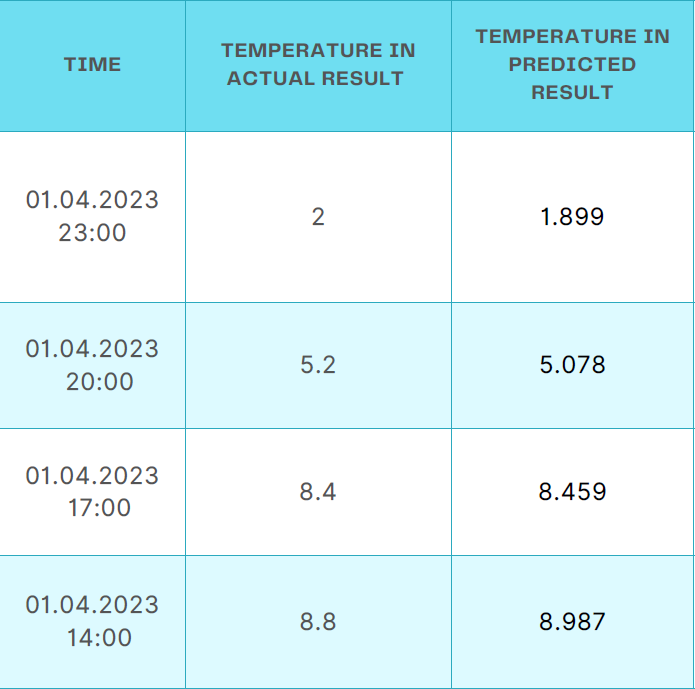
\includegraphics[width=0.4\textwidth]{assets/37}
	\caption*{Figure 2 -- Sample of real and predicted temperatures comparison}
\end{figure}

{\bfseries Conclusion.} This paper presents a detailed description of
constructing a machine learning model for weather numerical forecasting
based on open data, which is available to everyone. The main idea of the
research is to identify pairwise correlations between provided dataset
features and real data and to analyze multiple machine learning model
constructing approaches to predict weather in Almaty city region,
including region features (low pressure due to mountain region and
etc.).

In a result, we may forecast weather by provided data accurately and
potentially forecast the weather of other regions and future weather in
Almaty region as well. We can construct weather prediction applications
for numerical forecasting, but as for now we have some technical
limitations, like a lack of CPU to achieve better results in less
performing time.
\end{multicols}

\begin{center}
{\bfseries References}
\end{center}

\begin{noparindent}
1.P. Bauer, A. Thorpe, and G. Brunet, The quiet revolution of numerical
weather prediction.// Nature. 2015.-Vol.525 (7567).-P. 47-55.
DOI:10.1038/nature14956


2.M. Holmstrom, D. Liu, and C. Vo, Machine learning applied to weather
forecasting.// Meteorol. Appl.-2016.-Vol.10.- P.1-5, 2016. {[}Online{]}.
Available: \href{https://www.semanticscholar.org/paper/Machine-Learning-Applied-to-Weather-Forecasting-
Holmstrom-Liu/e2ed8aba53b4688808d57a0512496beb3548fc2c}{https://www.semanticscholar.org/}

3.A. Islam, S. Attwood, M. Braun, K. Kamp, and P. Aggarwal, Assessment
of capabilities, needs of communities, opportunities and limitations of
weather forecasting for coastal regions of Bangladesh. //WorldFish.-
2013. DOI 10.13140/RG.2.1.1706.6485

4.R. Pielke and M. Uliasz, Use of meteorological models as input to
regional and mesoscale air quality models-limitations and strengths,
Atmospheric Environment.-1998.-Vol.32 (8).-P.1455--1466. DOI

10.1016/S1352-2310(97)00140-4

5.S. Ravela, K. Emanuel, D. McLaughlin Data assimilation by field
alignment.// Physica D: Nonlinear Phenomena.-2007.- Vol. 230(1-2).-P.
127--145.DOI 10.1016/j.physd.2006.09.035

5.R. D. Thompson. Atmospheric processes and systems//Psychology Press.-
1998. -224 p.

DOI 10.4324/9780203015872

6.W. Shao Are actual weather and perceived weather the same?
understanding perceptions of local weather and their effects on risk
perceptions of global warming// Journal of Risk Research.- 2016.-Vol.19
(6).-P. 722-742.DOI10.1080/13669877.2014.1003956

7.C. Hahn, I. Garcia-Marti, J. Sugier, F. Emsley, A. L. Beaulant, L.
Oram, E. Strandberg, E. Lindgren, M. Sunter, and F. Ziska. Observations
from personal weather stations---eumetnet interests and experience.//
Climate.- 2022.-Vol.10(12),192 DOI 10.3390/cli10120192

8.H. Chen, Q. Zhang, and Y. Birkelund, Machine learning forecasts of
Scandinavian numerical weather prediction wind model residuals with
control theory for wind energy.// Energy Reports.-2022.-Vol.8.-P.
661-668. DOI 10.1016/j.egyr.2022.08.105

9.L. Donadio, J. Fang, and F. Port ́e-Agel, Numerical weather prediction
and artificial neural network coupling for wind energy forecast./
Energies.-2021.-Vol.4 (2), 338.

DOI 10.3390/en14020338

10.M.A.K. Azad, A. R. M. T. Islam, M. S. Rahman, and K. Ayen.
Development of novel hybrid machine learning models for monthly
thunderstorm frequency prediction over Bangladesh.//Natural
Hazards.-2021.-Vol.108.-P.110 -1135. DOI 10.1007/s11069-021-04722-9

11.K. Wilgan, W. Rohm, and J. Bosy, Multi-observation meteorological and
gnss data comparison with numerical weather prediction
model//Atmospheric Research.-2015.- Vol.156.- P. 29-42.- DOI
10.1016/j.atmosres.2014.12.011

12.N. Chen, Z. Qian, I. T. Nabney, and X. Meng, Wind power forecasts
using gaussian processes and numerical weather prediction //IEEE
Transactions on Power Systems.-2013.- Vol. 29(2).- P.656 - 665 DOI

10.1109/TPWRS.2013.2282366

13.Naveen L, Mohan H.S, Atmospheric Weather Prediction Using various
machine learning// 2019 3rd International Conference on Computing
Methodologies and Communication (ICCMC).

DOI 10.1109/ICCMC.2019.8819643

14.S. Madan, P. Kumar, S. Rawat, T. Choudhury. Analysis of Weather
Prediction using Machine Learning \& Big Data// 2018 International
Conference on Advances in Computing and Communication Engineering
(ICACCE). DOI 10.1109/ICACCE.2018.8441679

15.Vladimir M. Krasnopolsky, Michael S. Fox-Rabinovitz, Complex hybrid
models combining deterministic and machine learning components for
numerical climate modeling and weather prediction// Neural Networks.-
2006.- Vol.19(2).- P.122-134 DOI 10.1016/j.neunet.2006.01.002

16.G. Verma, P. Mittal, S. Farheen. Real Time Weather Prediction System
Using IOT and Machine Learning.// 2020 6th International Conference on
Signal Processing and Communication (ICSC).

DOI 10.1109/ICSC48311.2020.9182766

17.Xiaoli Ren, Xiaoyong Li, Kaijun Ren, Junqiang Song, Zichen Xu, Kefeng
Deng, Xiang Wang, Deep Learning-Based Weather Prediction: A Survey// Big
Data Research/- 2021.-Vol. 23, 100178.

DOI 10.1016/j.bdr.2020.100178

18.K.M.S.A. Hennayake, R. Dinalankara, D. Y. Mudunkotuwa, Machine
Learning Based Weather Prediction Model for Short Term Weather
Prediction in Sri Lanka.// 2021 10th International Conference on
Information and Automation for Sustainability (ICIAfS). DOI
10.1109/ICIAfS52090.2021.9606077
\end{noparindent}

\emph{{\bfseries Information about authors}}

\begin{noparindent}
Kair D.- Kazakh-British Technical University, Almaty, Kazakhstan,
e-mail: danikkair@gmail.com
\end{noparindent}

\emph{{\bfseries Сведения об авторе}}

\begin{noparindent}
Каир Д.- Казахстанско-Британский Технический Университет,Алматы,
Казахстан, e-mail:

danikkair@gmail.com
\end{noparindent}
